\documentclass[10pt]{article}
\usepackage[a4paper, total={7in,10in}]{geometry}
\usepackage{hyperref}
\usepackage{siunitx}
\usepackage{graphicx}
\usepackage{caption}
\usepackage[backend=biber]{biblatex}
\addbibresource{report.bib}

%opening
\title{EP2420 Project 2 - Forecasting Service Metrics}
\author{André Silva}
\begin{document}

\maketitle

\section*{Task I}
\label{sec:1}

In this task we use Linear Regression~\cite{LR} to predict, not the current state of a service metric, but the future states of said metric.

First, we pre-process the trace, standardizing along each column and removing outliers that deviate more than $40\sigma$. We also apply tree-based feature selection, using 10 estimators, to get the top $16$ features.

After this, we split the trace into training and test sets, and then transform them into new datasets that follow the structure $([x^{(t-l)},...,x^{(t)}],[y^{(t)},...,y^{(t+h)}])$. As we are using analyzing \textit{KV periodic}~\cite{9012741}, our step size (i.e. time between each sample of a sequence), is $1$ second.

We then perform an experiment to study the impact of $l$ on the accuracy of a model and its predictions of $0...10$ steps into the future by building $11$ different Linear Regression~\cite{LR} models with $l\in\{0,...,10\}$. The results can be found below in Figure $\ref{fig:1}$.

\begin{figure}[h!]
    \centering
    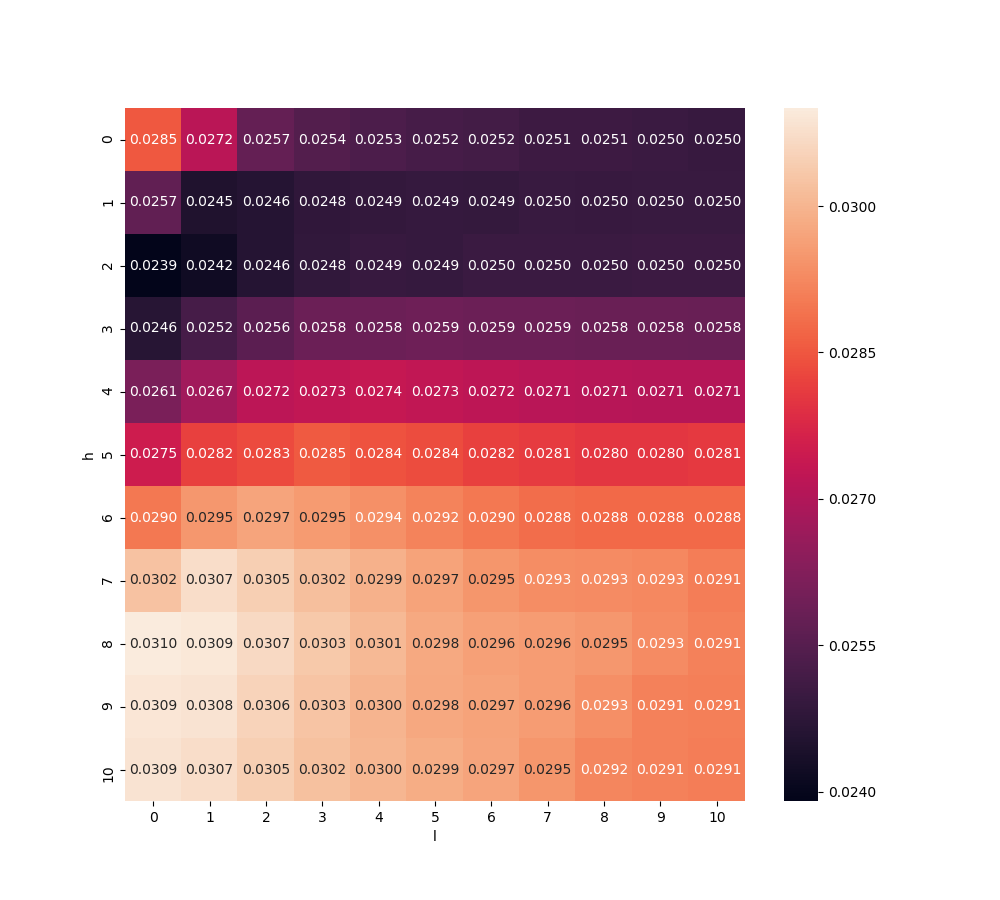
\includegraphics[width=0.75\textwidth,height=\textheight,keepaspectratio]{../result/project2/nmae_heatmap.png}
    \caption{Heat-map of \textsc{NMAE} for each Linear Regressor with $l\in\{0,...,10\}$ when predicting $y^{(t+h)}$}
    \label{fig:1}
\end{figure}

Figure \ref{fig:1} shows us the \textsc{NMAE} of each model when predicting $y^{(t+h)}$. Rows represent the time horizon $h = 0,...,10$ and columns represent the lag $l = 0,...,10$. The color gradient of the heat-map allows us to visualize and extract conclusions better than if we used a normal table.

When we analyze the results by looking at each row we notice that, in most cases, the \textsc{NMAE} decreases as we increase $l$. On the other hand, when we look at each column, we see that the \textsc{NMAE} increases as we increase $h$. Both these events are, intuitively, expected. When we increase $l$, we are providing more information, or context, to the model, so we expect better predictions. When we increase $h$, we are asking for a value that is more distant in time, and so, harder to predict.

This being said, we can also see that, when predicting $h = 1,..,7$, the \textsc{NMAE} don't monotonically decrease, when we increase $l$ from $0$, as expected. An explanation to this might be the fact that we built $11$ different models, as opposed to $11^2$ models, and so $y^{(t+h)}$ predictions are influenced by the noise of unused predictions. Another possible explanation could be that the current state of the system ($l=0$) can better predict the near future ($h>0$) than the actual current state ($h=0$), as system metric variations only have an impact on users after a certain time.


\printbibliography

\end{document}
